For instance, the modular aum described above
for the Sanskrit example [sanskrit.aut] generates the following code :

\begin{verbatim}
module Automata (Auto : sig type auto = 'a; end) =
   struct
    type auto_vect =
      { epsilon_aum : Auto.auto;
        noun : Auto.auto;
        root : Auto.auto;
        unde : Auto.auto;
        abso : Auto.auto;
        iic : Auto.auto;
        iiv : Auto.auto;
        auxi : Auto.auto;
        ifc : Auto.auto;
        prev : Auto.auto }
    ;
    module Disp (Fsm : sig value autos : auto_vect; end) =
      struct
        type phase =
          [ Init
          | Iic1
          | Noun
          | Iic2
          | Ifc
          | Prev1
          | Root
          | Iiv
          | Auxi
          | Prev2
          | Abso
          | Unde ]
        ;
        value transducer =
          fun
          [ Init -> Fsm.autos.empty_aum
          | Iic1 -> Fsm.autos.iic
          | Noun -> Fsm.autos.noun
          | Iic2 -> Fsm.autos.iic
          | Ifc -> Fsm.autos.ifc
          | Prev1 -> Fsm.autos.prev
          | Root -> Fsm.autos.root
          | Iiv -> Fsm.autos.iiv
          | Auxi -> Fsm.autos.auxi
          | Prev2 -> Fsm.autos.prev
          | Abso -> Fsm.autos.abso
          | Unde -> Fsm.autos.unde ]
        ;
        value dispatch =
          fun
          [ Init -> [Iic1; Noun; Iic2; Prev1; Root; Iiv; Prev2; Unde]
          | Iic1 -> [Iic1; Noun]
          | Noun -> [Iic1; Noun; Iic2; Prev1; Root; Iiv; Prev2; Unde]
          | Iic2 -> [Iic2; Ifc]
          | Ifc -> [Iic1; Noun; Iic2; Prev1; Root; Iiv; Prev2; Unde]
          | Prev1 -> [Root]
          | Root -> [Iic1; Noun; Iic2; Prev1; Root; Iiv; Prev2; Unde]
          | Iiv -> [Auxi]
          | Auxi -> [Iic1; Noun; Iic2; Prev1; Root; Iiv; Prev2; Unde]
          | Prev2 -> [Abso]
          | Abso -> [Iic1; Noun; Iic2; Prev1; Root; Iiv; Prev2; Unde]
          | Unde -> [Iic1; Noun; Iic2; Prev1; Root; Iiv; Prev2; Unde] ]
        ;
        value initial = Init;
        value terminal phase =
          List.mem phase [Noun; Ifc; Root; Auxi; Abso; Unde]
        ;
      end
    ;
  end
;
\end{verbatim}

Here is the resulting local automaton (adding empty nodes S, Subst, Verb,
Invar and Accept for better reading):
\begin{center} 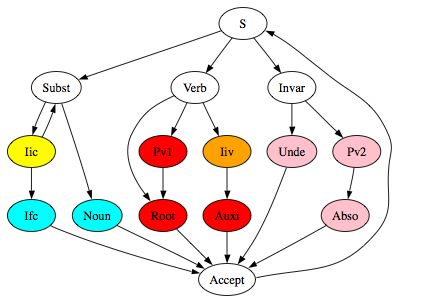
\includegraphics[width=11cm]{skt} \end{center} % comment-out for html

\section{Producing the engine}

We now have all the pieces to connect our dispatch plug-in to the generic reactive
engine, parameterized by the automata vector provided by the user for recognizing the
various phases. Let us give a concrete example. 

Given the {\it automata} functor corresponding to Sanskrit
morphology in a {\it Sanskrit\_dispatch} module, we show how to
link it to the {\it Reactt} functor in order to produce a Sanskrit engine generator: 
